%%%%%%%%%%%%%%%%%%%%%%%%%%%%%%%%%%%%%%%%%%%%%%%%%%%%%%%%%%%%%%%%%%%%%%%%%%
%
% StAssociationMaker - User Guide and Reference Manual -- LaTeX Source
%
% $Id: StAssociationMaker.tex,v 1.4 2000/02/15 01:28:25 calderon Exp $
%
% Authors:Michael A. Lisa
%         Thomas S. Ullrich
%         Manuel Calderon de la Barca Sanchez
%
%%%%%%%%%%%%%%%%%%%%%%%%%%%%%%%%%%%%%%%%%%%%%%%%%%%%%%%%%%%%%%%%%%%%%%%%%%
%
% Notes to the authors:
%
% - A template for a class reference is at the end of this file.
% - Wrap all names functions with \name{}
% - All code, examples, prototypes in \verb+ ... +\\
%   or \begin{verbatim} ... \end{verbatim}
% - Use \StAssociationMaker if you refer to the package itself (not the class)
%
% This file is best edit with xemacs and the 'Function' package loaded.
%
%%%%%%%%%%%%%%%%%%%%%%%%%%%%%%%%%%%%%%%%%%%%%%%%%%%%%%%%%%%%%%%%%%%%%%%%%%
%
% $Log: StAssociationMaker.tex,v $
% Revision 1.4  2000/02/15 01:28:25  calderon
% Updated first half of documentation,
% still more to do...
%
% Revision 1.3  1999/07/23 00:15:38  calderon
% Corrected documentation about macro location, and current libraries where StAssociationMaker runs
%
%
%%%%%%%%%%%%%%%%%%%%%%%%%%%%%%%%%%%%%%%%%%%%%%%%%%%%%%%%%%%%%%%%%%%%%%%%%%
\documentclass[twoside]{article}

\parindent 0pt
\parskip 6pt
\advance\textwidth by 80pt%
\advance\evensidemargin by -80pt%

\usepackage{graphicx}
\usepackage{psboxit}
\usepackage{amsmath}
\usepackage{amssymb}
\usepackage{amsfonts}
\usepackage{fancyhdr}
\usepackage{times}
\usepackage{verbatim}
\usepackage{makeidx}

\PScommands      % init boxit
\makeindex

%%%%%%%%%%%%%%%%%%%%%%%%%%%%%%%%%%%%%%%%%%%%%%%%%%%%%%%%%%%%%%%%%%%%
%
% Define header and footer style
%
%%%%%%%%%%%%%%%%%%%%%%%%%%%%%%%%%%%%%%%%%%%%%%%%%%%%%%%%%%%%%%%%%%%%
\pagestyle{fancyplain}
\rhead[\fancyplain{}{\bfseries\leftmark}]
      {\fancyplain{}{\bfseries\rightmark}}
\lhead[\fancyplain{}{\bfseries\rightmark}]
      {\fancyplain{}{\bfseries\leftmark}}
\rfoot[{}]{\fancyplain{}{\bfseries\thepage}}
\lfoot[\fancyplain{}{\bfseries\thepage}]{}
\cfoot{}

%%%%%%%%%%%%%%%%%%%%%%%%%%%%%%%%%%%%%%%%%%%%%%%%%%%%%%%%%%%%%%%%%%%%
%
% Typographic Conventions
%
%%%%%%%%%%%%%%%%%%%%%%%%%%%%%%%%%%%%%%%%%%%%%%%%%%%%%%%%%%%%%%%%%%%%
\newcommand{\name}[1]{\textsl{#1}}%  class-, function-, package names
\newcommand{\StEvent}{\textsf{StEvent}}
\newcommand{\StMcEvent}{\textsf{StMcEvent}}
\newcommand{\StAssociationMaker}{\textsf{StAssociationMaker}}
\newcommand{\StMcAnalysisMaker}{\textsf{StMcAnalysisMaker}}

%%%%%%%%%%%%%%%%%%%%%%%%%%%%%%%%%%%%%%%%%%%%%%%%%%%%%%%%%%%%%%%%%%%%
%
% Define multiline labels for class reference
%
%%%%%%%%%%%%%%%%%%%%%%%%%%%%%%%%%%%%%%%%%%%%%%%%%%%%%%%%%%%%%%%%%%%%
\newcommand{\entrylabel}[1]{\mbox{\textbf{{#1}}}\hfil}%
\newenvironment{entry}
{\begin{list}{}%
    {\renewcommand{\makelabel}{\entrylabel}%
     \setlength{\labelwidth}{90pt}%
     \setlength{\leftmargin}{\labelwidth}
     \advance\leftmargin by \labelsep%
    }%
}%
{\end{list}}

\newcommand{\Entrylabel}[1]%
{\raisebox{0pt}[1ex][0pt]{\makebox[\labelwidth][l]%
    {\parbox[t]{\labelwidth}{\hspace{0pt}\textbf{{#1}}}}}}
\newenvironment{Entry}%
{\renewcommand{\entrylabel}{\Entrylabel}\begin{entry}}%
  {\end{entry}}

\begin{document}

%%%%%%%%%%%%%%%%%%%%%%%%%%%%%%%%%%%%%%%%%%%%%%%%%%%%%%%%%%%%%%%%%%%%
%
%    Title page
%
%%%%%%%%%%%%%%%%%%%%%%%%%%%%%%%%%%%%%%%%%%%%%%%%%%%%%%%%%%%%%%%%%%%%
\begin{titlepage}
\pagestyle{empty}
\vspace*{-35mm}
\begin{center}
  \mbox{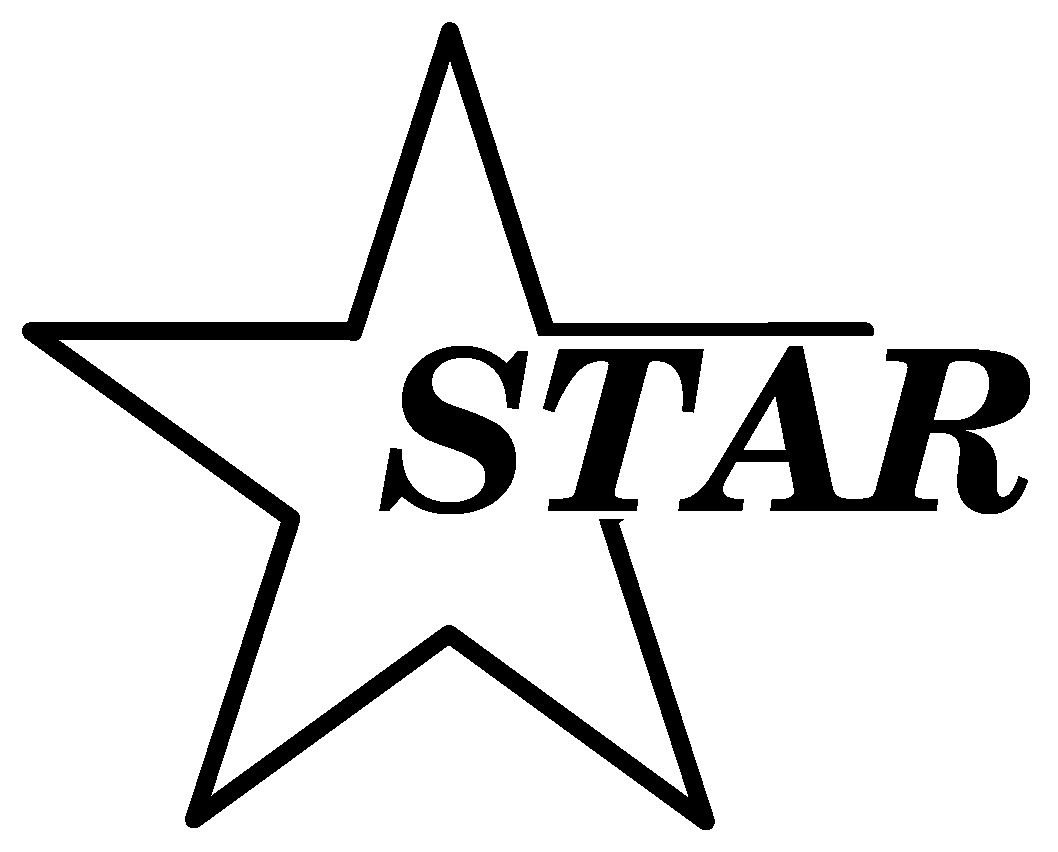
\includegraphics[width=2cm]{StarIcon.eps}}
  {\Large\bf STAR Offline Library Long Writeup}
  \hfill\mbox{}\\[3cm]
  \mbox{\includegraphics[width=\textwidth]{StAssociationMakerTitle.eps}}
  \hfill\mbox{}\\[3cm]
  {\LARGE User Guide and Reference Manual}\\[2cm]
  {\LARGE $  $}  \\[5mm] % replaced by cvs with current revision
  {\LARGE $  $}  % replaced by cvs with current revision
  \vfill
\end{center}
\cleardoublepage
\end{titlepage}
\pagenumbering{roman}

%%%%%%%%%%%%%%%%%%%%%%%%%%%%%%%%%%%%%%%%%%%%%%%%%%%%%%%%%%%%%%%%%%%%
%
%    Table of contents
%
%%%%%%%%%%%%%%%%%%%%%%%%%%%%%%%%%%%%%%%%%%%%%%%%%%%%%%%%%%%%%%%%%%%%
\tableofcontents
\cleardoublepage

%%%%%%%%%%%%%%%%%%%%%%%%%%%%%%%%%%%%%%%%%%%%%%%%%%%%%%%%%%%%%%%%%%%%
%
%    User Guide
%
%%%%%%%%%%%%%%%%%%%%%%%%%%%%%%%%%%%%%%%%%%%%%%%%%%%%%%%%%%%%%%%%%%%%
\pagenumbering{arabic}
\part{User Guide}
\clearpage

%%%%%%%%%%%%%%%%%%%%%%%%%%%%%%%%%%%%%%%%%%%%%%%%%%%%%%%%%%%%%%%%%%%%

\section{Introduction}

\StAssociationMaker\footnote{We will adopt the convention used in \StEvent\ 
    and write \StMcEvent\ when we refer to the package and
    \name{StMcEvent} when we refer to the class.} is a package that
uses the functionality of \StEvent\ and \StMcEvent\ together in order
to have reconstructed and Monte Carlo information handy.
The package is meant to be called in a chain after
both \StEvent\ and \StMcEvent\ have been loaded
in a ROOT session for a given event.  
\index{StAssociationMaker}
The aim of \StAssociationMaker\ is to establish the relationships, based
on certain criteria, between the reconstructed and Monte Carlo information.
In this way,
users can easily check whether a particular reconstructed hit or
track came from a Monte Carlo object, and directly obtain the associated Monte
Carlo hit or track so that an assessment of the quality of the
data can be made.

\clearpage

%%%%%%%%%%%%%%%%%%%%%%%%%%%%%%%%%%%%%%%%%%%%%%%%%%%%%%%%%%%%%%%%%%%%

\section{How to read this document}

This document is divided in two parts, a user guide and a
reference manual. The first part is the main part, since although
the package contains several classes, the only class that is designed
for general use is \name{StAssociationMaker}.  Apart from the usual
methods provided for makers, this class has only a few additional methods
for general use: the methods to access the multimaps.  The navigation and
use of \StEvent\ and \StMcEvent\ are described in their respective
documentation.
This manual will cover these methods, and how to
use the package.  The user guide will also provide an explanation of
the \StMcAnalysisMaker\ package.  This additional package is basically
a working example of how to do some basic histograms from the multimaps
built by the Association Maker.  The class reference will be kept short for the
reasons described above.
In addition, a section describing the main features of the \name{multimap} class
will also be provided.  Because \StAssociationMaker\ relies so heavily on
multimaps, giving a brief description of their idea and usage is
a necessary item in the documentation.

It remains true that understanding the various
examples certainly is the best way to get started. In this case,
\StMcAnalysisMaker\ is actually a working example, and many of the
things discussed here can be seen working ``live'' in this package.  To make
sure that it is working, one needs just to 
run the macro \name{StAssociator.C} at the root4star prompt.  
More information will be given
later on actually checking it out and modifying for your purposes \ref{sec:howto}.
%%%%%%%%%%%%%%%%%%%%%%%%%%%%%%%%%%%%%%%%%%%%%%%%%%%%%%%%%%%%%%%%%%%%

\section{Further documentation}
\label{sec:furtherdoc}

\StAssociationMaker\ makes use of various classes from the StarClassLibrary (SCL).
To obtain the SCL documentation perform the following steps:
\begin{enumerate}
  \item Obtain an \name{afs} token: \name{klog -cell rhic}.
  \item Make sure \name{\$CVSROOT} is set properly: \\ %%$
	(i.e.~\name{CVSROOT = /afs/rhic/star/packages/repository})
  \item Check-out the SCL into your current working directory:\\
    \name{cvs checkout StRoot/StarClassLibrary}
  \item Go to the directory containing the documentation:\\
    \name{cd StRoot/StarClassLibrary/doc/tex}
  \item Create the PostScript document \name{StarClassLibrary.ps}:\\
    \name{make}
\end{enumerate}
\index{SCL} \index{StarClassLibrary}

%%%%%%%%%%%%%%%%%%%%%%%%%%%%%%%%%%%%%%%%%%%%%%%%%%%%%%%%%%%%%%%%%%%%

\section{Getting \StAssociationMaker\ Sources}  \index{Getting StAssociationMaker sources}

To access the complete source code proceed as follows:

\StAssociationMaker\ is under {\bf CVS} control at BNL.  It can
be accessed via \name{afs}: \index{afs} \index{CVS} \index{CVSROOT}
\begin{enumerate}
  \item Obtain an \name{afs} token: \name{klog -cell rhic}.
  \item Make sure \name{\$CVSROOT} is set properly:\\ %%$
    (i.e.~\name{CVSROOT = /afs/rhic/star/packages/repository})
  \item Check-out package into your current working directory:\\
    \name{cvs checkout StRoot/StAssociationMaker}
  \item Check-out the examples
    \name{cvs checkout StRoot/StMcAnalysisMaker}
  \item Copy the macro your current working directory: \\
    \name{cp \$STAR/StRoot/macros/examples/StAssociator.C /.} %$
\end{enumerate}

%%%%%%%%%%%%%%%%%%%%%%%%%%%%%%%%%%%%%%%%%%%%%%%%%%%%%%%%%%%%%%%%%%%%

\section{Multimaps \& the Standard Containers}
\label{sec:Multimaps}
\index{multimap}
The definition of a multimap is not too long.
A multimap \footnote{For reference look in Stroustrup's C++ book, 3d Ed. pp. 484-490}
is a type of Standard Template Library associative container.
that allows for duplicate keys.  Now, initially, this definition doesn't
say much, unless you're already a C++ guru and know exactly what each part of the
definition means.  So I'll try to explain it little by little.  Then we'll
see how it all falls together.
The Standard Template Library (or STL) is a repository of several very useful
classes that can make programming a whole lot easier.  A few of the things
provided by the Standard Library are \textit{containers}, \textit{algorithms},
\textit{diagnostic} classes, \textit{string} handling classes, \textit{input/output} classes, and some
others.  As can be imagined, there is enough in the
Standard Library to warrant several books worth of documentation, which I don't
want to get into.  There are quite a few tutorials on the web about it also.  Part III
of Stroustrup's C++ book is totally devoted to the Standard Library, which is an
excellent starting point for more information.


The multimap is part of the STL, as one if the containers it provides.  There are
several containers with different features.  Examples	
are \name{lists}, \name{vectors}, and associative arrays like \name{map} and of
course \name{multimap}.  The C++ standard library
      containers were designed to meet 2 criteria: to provide as much freedom
      as possible in the design of individual containers and at the same
      time to provide a common interface to users.  This allows to make
      each container as efficient as possible for its intended use but
      still enable users to write code that is independent of the
      particular container being used.
      The standard library defines two kinds of containers: sequences and
      associative containers.  A key idea for the standard containers is that
      they should be logically interchangeable wherever reasonable.  Users can
      then choose between them depending on efficiency concerns and the
      need for specialized operations.  For example, if lookup based on
      a key is common, a \name{map} can be used.  If general list operations
      dominate, a \name{list} can be used.  If many additions and removals of
      elements occur at the ends of the container, a \name{deque} (double-ended
      queue), a \name{stack}, or a \name{queue} should be considered.

A first idea of what a \name{map} is can be ``a fast lookup table''.  You have entries
like in a \name{vector} container.  The difference is that every entry is a PAIR of
things.  
That is, a map can be thought of as a collection of pairs of
objects that are queried based on the first
element of the pair (the KEY). \index{KEY for a multimap}
The other element of the pair is referred to as the associated VALUE.

My favorite example to  illustrate
      the concept
      in a more familiar context, is to think of a phonebook.
The idea of a phonebook is
      that it
      contains people's phone numbers.  Simple.  Now, in the language we just learned,
      a phonebook is an associative
      container between a
      character string (a person's name) and an integer (the person's phone number).
      To use a
      phonebook,
      one looks up a person's name and reads off the associated phone number.  The character
      string representing the name is the "key", and the phone number is the key's
      associated "value".  

The difference between a multimap and a map is that the multimap allows for
several entries having the same key, whereas in a map no 2 entries can have the same
key.
This means that if a phonebook were a \name{map},
      then each person would only
      be able to have one phone number. Note that the phone number could be shared between
      people
      (only the keys
      are unique).  A \name{multimap}, on the other hand,
      allows multiple keys.  This means that if a phonebook were a
\name{multimap}, then everyone
      could have
      as many phone numbers as they pleased.

      One thing that help to picture the map and the multimap is the following.
      Recall the definition is that they are "associative containers of
      pairs of
      objects".  You can always think of a vector as an array.  So if you have
      a \verb+vector<int>+ then you can picture it like this:
\begin{center}
      \begin{tabular}{|c|c|c|c|c|c|c|}
	  \hline
	  \textbf{Vector}: & 1 & 2 & 5 & 17 & 20 & 25 \\ \hline
      \end{tabular}
\end{center}

    So the first element is 1, the second is 2 and so on.  Now, a map is a
    container of PAIRS of objects.  The 2 objects can be anything, (i.e. the
    PAIR class is also a template.)  So a phonebook would be, for example, 
    a
    
    \texttt{map<string,int, less<string> >}

I would picture it like this:
\begin{center}
\begin{tabular}{cc}
  \begin{tabular}{|c|}	
	\hline
	   \textbf{Map}:   \\ \hline
	  ("Brian",2034322043)  \\ \hline
	  ("Manuel",6313448342) \\ \hline
	  ("Thomas",2034325829) \\ \hline
	  \\ \hline
\end{tabular} &
  \begin{tabular}{l}
	  \\
	$\longleftarrow$ \verb+phonebook.begin()+ \\
	  \\
	  \\
	$\longleftarrow$ \verb+phonebook.end()+ \\
  \end{tabular}


\end{tabular}
\end{center}

    Now, the 'key' here would be the \texttt{string}, and the 'value' the
    \texttt{int} representing the phone
    number.  Since it is a map, keys are unique.  This means that there
    will only be one entry for each string.  
    If I say:
    
    \begin{verbatim}
      phonebook["Manuel"] = 2034325637;
    \end{verbatim}
    
    the entry for "Manuel" will be overwritten.
    
    Note that I can say 
    
    \begin{verbatim}
      phonebook["Thomas"] = phonebook["Manuel"];
    \end{verbatim}
    
    and I'll overwrite Thomas's phone number with mine.  The 'values' 
    can be repeated.

    We see here that a map
    supports indexing.  Since there is one entry for each key (and only one),
    it is unambiguous which entry one wants, so we can use the key as an index.
    A multimap doesn't support indexing,
    because there is still the ambiguity of having multiple entries.
    If we made the phonebook a
    
    \begin{verbatim}
      multimap<string, int, less<string> > 
    \end{verbatim}
    
      then we could have

\begin{center}
\begin{tabular}{cc}
  \begin{tabular}{|c|}	
	\hline
	   \textbf{Multimap}:   \\ \hline
	  ("Brian",2034322043)  \\ \hline
	  ("Manuel",6313448342) \\ \hline
	  ("Manuel",2034325637) \\ \hline
	  ("Thomas",2034325829) \\ \hline
  \end{tabular} &
  \begin{tabular}{l}
	 \\
	 \\
	$\longleftarrow$ \verb+phonebook.lower_bound(``Manuel'');+ \\
	 \\
	$\longleftarrow$ \verb+phonebook.upper_bound(``Manuel'');+ \\
  \end{tabular}


\end{tabular}
\end{center}

Because simple
subscripting by keys (like an array) is \textbf{not} supported for a multimap,
the main way to access
the multiple associated values given to a particular key is through iterators.
\index{iterators}
Iterators can be thought of as a pointer to an element of a container which
allow one to navigate through it.  For example, for the \name{list} container,
(or \name{vector} or pretty much any STL container) one can loop through
all the elements by doing

\begin{footnotesize}
\begin{verbatim}
   list<int> myList;
   // something is done and the list is filled

   list<int>::iterator listIter;
   for (listIter = myList.begin(); listIter != myList.end(); listIter++){
       // do something with the entry
   }
\end{verbatim}
\end{footnotesize}

The \texttt{begin()} method returns an
iterator to the first element of the container, \index{begin()}
and the \texttt{end()} method returns an \index{end()}
iterator to the last-plus-one element of the container.  So to iterate through
a container, we need 2 iterators because you don't know a priori how many entries there are.
One will be the starting point
and the other the end point.
For iterating through the entries with a common key, we use lower\_bound and upper\_bound.
You can think of them as the equivalent to
\texttt{vector.begin();} and
\texttt{vector.end();}

The use of iterators to navigate through a sequence of entries with a similar key is
possible because all the entries in the multimap are ordered according to some
criterion.  The entries with a similar key are then placed right next to each
other in the container.  In the phonebook example, all the entries for ``Manuel''
are placed next to each other.  In the example, we took the default comparison
for strings, which is just alphabetical order.  That is where the \verb+less<string>+
part comes in, for the example phonebook.  One has to specify a comparison, if the
compiler doesn't take default template arguments.  And even if it does, for other
user defined classes one
has to provide a custom made ordering.  This custom made ordering can also be
implemented for a built in class, if need be.
The bottom line is that the elements of the
multimap with the same key end up next to each other, ready to be looped over
with the iterators.


      It is important to stress that every entry in the multimap is a key-value pair,
      regardless of whether the key has appeared before.  This means that there is some
      redundancy.  If you loop over a sequence of entries using lower\_bound and
      upper\_bound, ALL of the entries in that sequence will have the same key:

\begin{center}
\begin{tabular}{cc}
  \begin{tabular}{|c|}	
	\hline
	   \textbf{Multimap}:   \\ \hline
	  ("Manuel",631...) \\ \hline
	  ("Manuel",203...) \\ \hline
	  ("Manuel",212...) \\ \hline
  \end{tabular} &
  \begin{tabular}{l}
	 \\
	$\longleftarrow$ first entry with key = ``Manuel'' \\
	$\longleftarrow$ second entry, same {\bf key}, different {\bf value} \\
	$\longleftarrow$ third entry, etc. \\
  \end{tabular}


\end{tabular}
\end{center}

For a multimap, then, \name{lower\_bound(k)} and \name{upper\_bound(k)} give the beginning
and end of the subsequence of elements of the map that have the key ``k''.  However,
as Stroustrup says, doing 2 operations all the time is neither elegant nor efficient.  The
operation \name{equal\_range(k)} is provided to deliver both.  For examples of this usage 
refer to sec.~\ref{sec:howto}. 

The multimaps used in \StAssociationMaker\ 
keep a relationship between the reconstructed \StEvent\ objects and Monte Carlo
\StMcEvent\ objects.  This
relationship is established starting from the hit information and building up
from there.

The following multimaps are now implemented in \StAssociationMaker :

    \begin{itemize}
      \item TPC Hits
      \item SVT Hits
      \item FTPC Hits
      \item Tracks  (using all the previous hit multimaps)
      \item Kink Vertices 
      \item V0 Vertices 
      \item Xi Vertices 
      
    \end{itemize}
The association is made based on criteria given by the user.  These criteria are
established at runtime, and the user controls them at the macro level.

The criterion for associating a given reconstructed hit to a \index{Hit association}
Monte Carlo hit is based on their spatial proximity, in the global coordinate system.

Once the hit associations are made, the criterion for associating a
reconstructed track to a Monte Carlo track is \index{Track association}
based on the number of hits they have in common.
This means that to build the Track Multimap, the Hit Multimaps are used.
    The defaults are:
\begin{verbatim}
    TPC Cuts
    X Cut    : 5 mm
    Y Cut    : 5 mm
    Z Cut    : 2 mm
    Required TPC Hits for Associating Tracks : 3
    SVT Cuts
    X Cut    : 1 mm
    Y Cut    : 1 mm
    Z Cut    : 1 mm
    Required SVT Hits for Associating Tracks : 1
    FTPC Cuts
    R Cut    : 3 mm
    Phi Cut  : 5 degrees
    Required FTPC Hits for Associating Tracks : 3
\end{verbatim}
These numbers are supposed to be much larger than the intrinsic resolution
of the detectors.  The idea is
to keep these numbers loose so the map would really rule out bad associations but keep
enough objects in the multimap to make further analysis downstream.

In addition, this version of \StAssociationMaker also provides 2 multimaps
for each of the objects above.  That is, there are 2 multimaps for
TPC Hits, 2 multimaps for SVT Hits, and so on.  One of the multimaps
uses the {\bf reconstructed} objects from \StEvent\ as keys, and the
other multimap uses the {\bf Monte Carlo} objects from \StMcEvent\ as
keys.  Even though this might appear redundant at first (there is a one to one correspondence
between the entries in the reconstructed map and the entries in the monte carlo map)
remember that one can only lookup entries based on the key.  There are cases where
we might want to lookup based on the reconstructed objects, and there are cases
where we will want to use the monte carlo objects.  Having 2 maps 
allows to find an association in both directions.

Almost all
multimaps are just between a reconstructed object and a monte carlo object.
The notable exception are the Track multimaps.
For the reconstructed track multimap, instead of just associating an
\name{StGlobalTrack} to an \name{StMcTrack}, we make the association between an
\name{StGlobalTrack} and an instance of an \name{StTrackPairInfo} class. \index{StTrackPairInfo}
This class has,
of course, a pointer to the associated \name{StMcTrack} but in additon has a member that
keeps track of the number of hits the 2 tracks have in common for each of the
detectors, and member functions that return the {\it percent} of hits in each
detector that are associated out of the total number of hits the track has.
This is done so that
later on one can make more stringent cuts on the tracks.  If any additional information
is needed, we would only need to modify the \name{StTrackPairInfo} class to accomodate it.
For the monte carlo track multimap, the ``value'' of the multimap is also the same
pointer to the \name{StTrackPairInfo} class.
This means, of course, that \name{StTrackPairInfo}
must also have a pointer to the associated \name{StGlobalTrack},
in addition to the \name{StMcTrack}.


We said that the default values of required hits in common, spatial proximity, etc.
can also be modified at the macro level.
The cuts are kept in an instance of the singleton class \name{StMcParameterDB}.  This
class is instantiated exactly once (hence the name ``singleton'') and the rest of
the classes in \StAssociationMaker\ look there to figure out the cut criteria.
For an example of how to change the cuts, look in the \name{StAssociator.C}
macro.


%%%%%%%%%%%%%%%%%%%%%%%%%%%%%%%%%%%%%%%%%%%%%%%%%%%%%%%%%%%%%%%%%%%%


\section{How to use it: StMcAnalysisMaker and StAssociator.C}
\label{sec:howto}
\index{StAssociator.C}
\index{StMcAnalysisMaker}
\index{root4star}
\index{ROOT files}
The procedure starting from scratch to run the provided 
example is just to run the macro in any directory.
The package should run in any platform and any version
of the library.
\begin{verbatim}
    ssh rcas6001
    starnew
    mkdir workdir
    cd workdir
    root4star
    .x StAssociator.C
\end{verbatim}

To get the code you can just check it out from the library.
Probably the one you'll want to check out and modify
is StMcAnalysisMaker, since it is filled with examples.
But one can certainly check out the Association Maker
to look at the source, which is always
the most up to date documentation of what is available.
\begin{verbatim}
    cvs co StRoot/StAssociationMaker
    cvs co StRoot/StMcAnalysisMaker
\end{verbatim}

You can edit the Analysis maker and then compile using cons.
\begin{verbatim}
    cons +StMcAnalysisMaker/
    cvs co StRoot/macros/examples/StAssociator.C  
    Edit the macro to use your maker, if you wisely renamed it before editing.
    root4star StAssociator.C
\end{verbatim}
\index{cons}
Note that to compile using cons, you don't need to give the exact name of the maker.
A substring works, but it will try to compile everything that matches the substring.
This means that if you have several packages checked out and you want to compile
them all, you can probably do

\verb!     cons +St!

and this will do the trick.

StAssociator.C can be found in \name{\$CVSROOT/StRoot/macros/examples/StAssociator.C}. %$%%%
To get it you must use \verb+cvs co+ command as above. The macro runs a 
chain consisting of four makers:
\begin{description}
\item[\name{StEventReaderMaker}:] loads StEvent
\item[\name{StMcEventMaker}:] loads StMcEvent
\item[\name{StAssociationMaker}:] creates the hit and track associations
\item[\name{StMcAnalysisMaker}:] Picks up the previous info. and analyzes it 
    (incorporates a few simple examples)
\end{description}

%%%%%%%%%%%%%%%%%%%

At the moment, it runs the chain on a ROOT file tree.  That is, it uses the DST
and GEANT braches of the files it finds in the directory.  Example invocation
is
\begin{footnotesize}
\begin{verbatim}
.x StAssociator.C(10,
    "/disk00000/star/test/new/tfs_Solaris/year_2a/psc0210_01_40evts.geant.root")

   processes 10 events from the specified file

\end{verbatim}
\end{footnotesize}

It takes the path to look for files from the specified file, but the files it
actually opens depend on
what branches are activated in the macro.
This is done inside the macro with the command \name{SetBranch}.


\subsection{StMcAnalysisMaker::Make()}
We will explain here the first example in
the \name{Make()} method of \name{StMcAnalysisMaker}, since this is the
part that most users will follow.
Recall that when \name{StMcAnalysisMaker::Make()} is called, the following should have already
happened:
\begin{enumerate}
\item \StEvent\ should be loaded in the chain.
\item \StMcEvent\ should be loaded in the chain.
\item \StAssociationMaker\ should have finished making associations.
\end{enumerate}

We need to access the packages and information that is already loaded.  This is done
by getting a pointer to \name{StEvent}, a pointer to \name{StMcEvent}, and a pointer
to \name{StAssociationMaker}:

\begin{verbatim}
    // Get the pointers we need, we have to use the titles we gave them in the
    // macro.  I just used the defaults.
    StEvent* rEvent = 0;
    rEvent = ((StEventMaker*) gStChain->Maker("events"))->event();
    StMcEvent* mEvent = 0;
    mEvent = ((StMcEventMaker*) gStChain->Maker("MCEvent"))->currentMcEvent();
    StAssociationMaker* assoc = 0;
    assoc = (StAssociationMaker*) gStChain->Maker("Associations");
\end{verbatim}

The pointer to \name{StAssociationMaker} then enables us to get the pointers to the
appropriate multimpas:

\begin{verbatim}

    tpcHitMapType* theHitMap = 0;
    theHitMap = assoc->tpcHitMap();
    trackMapType* theTrackMap = 0;
    theTrackMap = assoc->trackMap();

\end{verbatim}

The classes \name{tpcHitMapType} and \name{trackMapType} are the typedef's to the
appropriate multimaps.  \index{tpcHitMapType} \index{trackMapType} 
We see here that to get a the pointers to them we just need to call
the \name{StAssociationMaker::tpcHitMap()} and \name{StAssociationMaker::trackMap()} methods.

Once we have the pointers to the maps, we can start analyzing them.  The first example
in the maker shows how to check whether a particular reconstructed TPC Hit was associated
with a Monte Carlo hit. 

\begin{verbatim}

 // Example: look at hits associated with 1st REC hit in Tpc Hit collection.

 StTpcHit*     firstHit;
 firstHit = *( rEvent->tpcHitCollection()->begin() );
 cout << "Assigned First Hit: " << endl;
 cout << *firstHit << endl;
 cout << "This hit has " <<  theHitMap->count(firstHit);
 cout << " MC Hits associated with it."<< endl;

 // To get the associated hits of the first hit we use equal_range(key),
 // which returns 2 iterators, the lower bound and upper bound,
 // so that then we can loop over them.
    
 cout << "Position of First Rec. Hit and Associated (if any) MC Hit:" << endl;
 pair<tpcHitMapIter,tpcHitMapIter> hitBounds = theHitMap->equal_range(firstHit);

 for (tpcHitMapIter it=hitBounds.first; it!=hitBounds.second; ++it) {
    cout << "[" << (*it).first->position();
    cout << ", "<< (*it).second->position() << "]" << endl;
 }
\end{verbatim}

The other examples in the maker show
\begin{enumerate}
\item how to make a histogram using the Hit multimap
\item how to use an \name{StGlobalTrack} to get its partner in the Track multimap.
\item how to make a histogram using the Track multimap
\end{enumerate}

(Note that the histograms were defined in the header file as public data members.)

To play with it yourself you can pick up StMcAnalysisMaker and 
use it as a template for a Maker of your own that works with
StMcEvent:

\begin{verbatim}
    mkdir StRoot/StMyMcAnalysisMaker
    cp  $STAR/StRoot/StMcAnalysisMaker/* StRoot/StMyMcAnalysisMaker/                                   %$
    [edit]
    makel -C StRoot/StMyMcAnalysisMaker
    cvs co $CVSROOT/StRoot/macros/examples/StAssociator.C  (and edit to use your maker)                            %$
    root4star StAssociator.C
\end{verbatim}

%%%%%%%%%%%%%%%%%%%%%%%%%%%%%%%%%%%%%%%%%%%%%%%%%%%%%%%%%%%%%%%%%%%%


\section{Known Problems} \index{known problems (\StAssociationMaker\ )}

\StAssociationMaker\ is not yet complete.  
It has only been tested in new, SL99e.  We do not foresee
to make it work in dev (SL99f) since \StEvent\ itself is going through a major
overhaul.  The next version will be developed once the new \StEvent\
is in place, and also the changes in the g2t\_vertex table have been
implemented.

The FTPC and SVT associations between reconstructed and Monte Carlo
hits are not included presently (although the appropriate Collections are
filled by \name{StMcEventMaker} ). 
Also, \StAssociationMaker\ does not compile with SUN CC4.2 yet, because
that compiler has problems handling multimaps, and this is being worked on.


\clearpage

%%%%%%%%%%%%%%%%%%%%%%%%%%%%%%%%%%%%%%%%%%%%%%%%%%%%%%%%%%%%%%%%%%%%
%
%    Reference Manual
%
%%%%%%%%%%%%%%%%%%%%%%%%%%%%%%%%%%%%%%%%%%%%%%%%%%%%%%%%%%%%%%%%%%%%
\part{Reference Manual}
\label{refman}
\clearpage

%%%%%%%%%%%%%%%%%%%%%%%%%%%%%%%%%%%%%%%%%%%%%%%%%%%%%%%%%%%%%%%%%%%%

\section{Global Constants}

We use the constants defined in the two header files
\index{StarClassLibrary} \name{SystemOfUnits.h} and
\name{PhysicalConstants.h} which are part of the StarClassLibrary.
The types defined therein are used
throughout \StMcEvent\ .

%%%%%%%%%%%%%%%%%%%%%%%%%%%%%%%%%%%%%%%%%%%%%%%%%%%%%%%%%%%%%%%%%%%%


\section{Class Reference}
The classes which are currently implemented and available from the
STAR CVS repository are described in alphabetic order.  Only the
classes normally accessible to users are described.

\clearpage


%%%%%%%%%%%%%%%%%%%%%%%%%%%%%%%%%%%%%%%%%%%%%%%%%%%%%%%%%%%%%%%%%%%%
%
%    Reference: StAssociationMaker
%
%%%%%%%%%%%%%%%%%%%%%%%%%%%%%%%%%%%%%%%%%%%%%%%%%%%%%%%%%%%%%%%%%%%%
\subsection{StAssociationMaker}
\index{StAssociationMaker|textbf}
\index{event header}
\label{sec:StAssociationMaker}
\begin{Entry}
\item[Summary]
    \name{StAssociationMaker} is the main class in the \StAssociationMaker\ package.
    It aim is to create the multimaps, and to provide methods to access them. 

\item[Synopsis]
    \verb+#include "StAssociationMaker.h"+\\
    \verb+class StAssociationMaker;+\\

\item[Description]
    Objects of type \name{StAssociationMaker} are the entry point to the hit
    and track multimaps.
    From here one can navigate to (and access) quantities stored
    in them.  Of course, one normally needs to include the necessary
    \StEvent\ and \StMcEvent\ classes to use in one's own analysis maker.

\item[Persistence]
    None

\item[Related Classes]
    None

\item[Public\\ Constructors]
    \verb+StAssociationMaker(const char* name = "Associations",const char* title = "event/Associations");+\\
		       
    Maker constructor.

\item[Public Member\\ Functions]
    

    \verb+virtual void Clear(const char* opt="");+\\
    Deletes the multimaps and the single histogram data member.  Then calls standard Clear() for makers. 
    \index{Clear()}

    \verb+virtual Int_t Init();+\\
    Standard for makers. 
    \index{Init()}

    \verb+virtual Int_t Make();+\\
    Makes hit and track associations, i.e. builds the multimaps.
    \index{Make()}

    \verb+virtual Int_t Finish();+\\
    Standard for makers.
    \index{Finish()}

    \verb+tpcHitMapType* tpcHitMap();+\\
    Returns the pointer to the TPC Hit multimap.  This is the way to get access to
    the map from another maker.  Look in sec.~\ref{sec:howto}
    \index{tpcHitMap()}

    \verb+trackMapType* trackMap()+\\
    Returns the pointer to the Track multimap.  This is the way to get access to
    the map from another maker.  Look in sec.~\ref{sec:howto}
    \index{trackMap()}

\end{Entry}

%%%%%%%%%%%%%%%%%%%%%%%%%%%%%%%%%%%%%%%%%%%%%%%%%%%%%%%%%%%%%%%%%%%%
%
%    Reference: StMcParameterDB
%
%%%%%%%%%%%%%%%%%%%%%%%%%%%%%%%%%%%%%%%%%%%%%%%%%%%%%%%%%%%%%%%%%%%%
\subsection{StMcParameterDB}
\index{StMcParameterDB|textbf}
\label{sec:StMcParameterDB}
\begin{Entry}
\item[Summary]
    \name{StMcParameterDB} is a singleton class that keeps track
    of the cuts to be used for making hit and track associations.
    If used, it should be called from the macro, so an include command
    should not be necessary since it is already included in
    \name{StAssociationMaker}.  

\item[Synopsis]
    \verb+#include "StMcParameterDB.hh"+\\
    \verb+class StMcParameterDB;+\\

\item[Description]
    To use it in the macro one just needs to get a pointer to the only instance
    of the class.  This is done through the StMcParameterDB::instance() method:
     \verb+StMcParameterDB* parameterDB = StMcParameterDB::instance();+\\

    One then uses this pointer to access the methods of the class.

\item[Persistence]
    None

\item[Related Classes]
    None

\item[Public\\ Constructors]
    None
    
    The class only has private constructors. The only access to it is through its member
    functions.

\item[Public Member\\ Functions]

    \verb+static StMcParameterDB* instance();+\\
    Returns a pointer to the only instance of the class.  This is the way to access the
    the class from another macri.  Look in \name{StAssociator.C} for an example.
    \index{instance()}

    \verb+double xCut() const;+\\
    Returns the present value of the cut in the x direction for hit associations.
    \index{xCut()}

    \verb+double zCut() const;+\\
    Returns the present value of the cut in the z direction for hit associations.
    \index{zCut()}

    \verb+unsigned int reqCommonHits() const;+\\
    Returns the present value of the cut in the number of common hits for track associations.
    \index{reqCommonHits()}

    \verb+void setXCut(double);+\\
    Sets the value of the cut in the x direction for hit associations.

    \verb+void setZCut(double);+\\
    Sets the value of the cut in the z direction for hit associations.

    \verb+void setReqCommonHits(unsigned int);+\\
    Sets the value of the cut in the number of common hits for track associations.

\end{Entry}


%%%%%%%%%%%%%%%%%%%%%%%%%%%%%%%%%%%%%%%%%%%%%%%%%%%%%%%%%%%%%%%%%%%%
%
%    Reference: StTrackPairInfo
%
%%%%%%%%%%%%%%%%%%%%%%%%%%%%%%%%%%%%%%%%%%%%%%%%%%%%%%%%%%%%%%%%%%%%
\subsection{StTrackPairInfo}
\index{StTrackPairInfo|textbf}
\label{sec:StTrackPairInfo}
\begin{Entry}
\item[Summary]
    \name{StTrackPairInfo} is the class that contains the information of the pair of
    a particular \name{StGlobalTrack}. It has as members the associated
    \name{StMcTrack} and the number of common hits beween the paired tracks.

\item[Synopsis]
    \verb+#include "StTrackPairInfo.hh"+\\
    \verb+class StTrackPairInfo;+\\

\item[Description]
    \name{StTrackPairInfo} provides a way to keep the information gained during the
    building of the multimap, like the number of common hits between tracks, for
    later use in the analysis.

\item[Persistence]
    None

\item[Related Classes]
    This class related to \name{StMcTrack} through composition, i.e. it
    contains a pointer to an
    \name{StMcTrack} as a member. 
    \index{StMcTrack}
    
\item[Public\\ Constructors]
    \verb+StTrackPairInfo(StMcTrack* t, unsigned int pings);+\\
    Constructs an instance of \name{StTrackPairInfo} with partner MC Track \name{t} and
    number of common hits \name{pings}.

\item[Public Member\\ Functions]
    \verb+StMcTrack* partnerMcTrack() const;+\\
    Returns a pointer to the \name{StMcTrack} paired with a particular \name{StGlobalTrack} used
    as a key in the Track map.

    \verb+unsigned int commonHits() const;+\\
    Number of common hits between the paired tracks.

    \verb+void setPartnerMcTrack(StMcTrack*);+\\
    Sets the partner track.  Should not normally be used, since this is taken care of
    during construction of the class.

    \verb+void setCommonHits(unsigned int);+\\
    Sets the number of common hits.  Should not normally be used, since this is taken care of
    during construction of the class.

\end{Entry}

%%%%%%%%%%%%%%%%%%%%%%%%%%%%%%%%%%%%%%%%%%%%%%%%%%%%%%%%%%%%%%%%%%%%
%
% The End
%
%%%%%%%%%%%%%%%%%%%%%%%%%%%%%%%%%%%%%%%%%%%%%%%%%%%%%%%%%%%%%%%%%%%%

\printindex

\end{document}
\bye
% The text following after this line is not included into the text

%
%  Template for reference section
%

%%%%%%%%%%%%%%%%%%%%%%%%%%%%%%%%%%%%%%%%%%%%%%%%%%%%%%%%%%%%%%%%%%%%
%
%    Reference: className
%
%%%%%%%%%%%%%%%%%%%%%%%%%%%%%%%%%%%%%%%%%%%%%%%%%%%%%%%%%%%%%%%%%%%%
\subsection{className}
\index{className|textbf}
\label{sec:className}
\begin{Entry}
\item[Summary]

\item[Synopsis]
    \verb+#include "className.hh"+\\
    \verb+class className;+\\

\item[Description]

\item[Persistence]
    None

\item[Related Classes]

\item[Public\\ Constructors]

\item[Public Member\\ Functions]

\item[Public Member\\ Operators]

\item[Public Functions]

\item[Public Operators]

\item[Examples]
{\footnotesize
\begin{verbatim}
//
//  What the example does
//

\end{verbatim}
}%footnotesize

\end{Entry}
